\documentclass{article}

\usepackage[utf8]{inputenc}
\usepackage[T1]{fontenc}

%%%%%
\usepackage{graphicx}
\usepackage{caption}
\usepackage{subcaption}

% lock figure into place (H option of \begin{figure})
\usepackage{float}
  
% wrapping text around figures
\usepackage{wrapfig}

\usepackage[english]{babel}

\usepackage{amsmath}
\usepackage{amssymb}
\usepackage{amsfonts}
\usepackage{amsopn}
\usepackage{braket}
\usepackage{bbm}
\usepackage{dsfont}
\usepackage{kpfonts}
\usepackage{amsthm}
% \usepackage{mathabx}

\parindent=0cm


% Various new commands that ease typesetting math even further
% \newcommand{\assign}{\ensuremath{\coloneq}}
% \newcommand{\rassign}{\ensuremath{\eqcolon}}
\newcommand{\assign}{\ensuremath{:=}}
\newcommand{\rassign}{\ensuremath{=:}}

\newcommand{\of}[1]{\ensuremath{\left( #1 \right)}}
\newcommand{\ofs}[1]{\ensuremath{\left( #1 \right)}}

\newcommand{\norm}[1]{\ensuremath{\| #1 \|}}

\newcommand{\tmop}[1]{\ensuremath{\operatorname{#1}}}

\newcommand{\id}{\ensuremath{\mathds{1}}}
% \newcommand{\id}{\ensuremath{I}}


\newcommand{\conj}[1]{\ensuremath{\overline{#1}}}

\newcommand{\T}{\ensuremath{{}^{\textnormal{T}}}}
\newcommand{\herm}{\ensuremath{{}^{\textnormal{H}}}}

\newcommand{\ft}[1]{\ensuremath{\mathcal{F}\left(#1\right)}}
\newcommand{\ift}[1]{\ensuremath{\mathcal{F}^{-1}\left(#1\right)}}

\newcommand{\fft}[1]{\ensuremath{\mathtt{FFT}\left(#1\right)}}
\newcommand{\ifft}[1]{\ensuremath{\mathtt{IFFT}\left(#1\right)}}

\newcommand{\dotp}[2]{\ensuremath{\langle #1 , #2 \rangle}}

\newcommand{\bigO}[1]{\ensuremath{\mathcal{O}\left( #1 \right)}}

\newcommand{\mat}[1]{\ensuremath{\mathbf{#1}}}

% multi-indices
\newcommand{\mindex}[1]{\ensuremath{\underline{#1}}}

% reprensents an array/vector of coefficients
\newcommand{\laplace}{\ensuremath{\operatorname{\Delta}}}

% EOF

 
\usepackage[ruled]{algorithm2e}

% Configure Algorithm2e
\DontPrintSemicolon
\SetKwInOut{Input}{Input}
\SetKwInOut{Output}{Output}

\def\code#1{\texttt{#1}}
\newtheorem{definition}{Definition}

\begin{document}

\section{Basic Shape}

A \(D\)-dimensional shape \(\mathfrak{K}\) is a set of \emph{unordered} D-dimensional integer-tuples, also referred to as \emph{nodes}.
A shape is suitable for our needs if it satisfies:
\[k \in \mathfrak{K} \Rightarrow \forall k^\star \preceq k \colon k^\star \in \mathfrak{K}\]
That means, if an arbitrary node is part of the shape, then all nodes in the backward cone are part of the shape too.

\subsection{Implementation}

\subsection{Shape Extension}

\begin{definition}
Given a basis shape \( \mathfrak{K} \), the shape extension
\( \overline{\mathfrak{K}} \) is defined by
\begin{equation}
\overline{\mathfrak{K}} := \mathfrak{K} \cup 
\left\{\underline{k}' \colon \underline{k}' = \underline{k} + \underline{e}^d 
\forall d \in \{1,\ldots,D\} \forall \underline{k} \in \mathfrak{K}\right\}
\end{equation}
where \( \underline{e}^d \) is the unit vector in direction \( d \).
\end{definition}

\begin{figure}[H]
  \begin{center}
    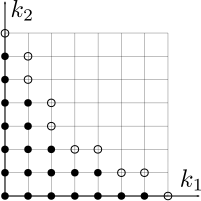
\includegraphics[width=0.5\linewidth]{shape_extension}
  \end{center}
  \caption{basic shape (filled bullets) and its extension (empty bullets)}
\end{figure}

\subsection{Shape Union}

\begin{definition}
Given the shapes \( \mathfrak{K}_1, \ldots \mathfrak{K}_N \), the union of these shapes
is defined by
\begin{equation}
union(\mathfrak{K}_1,\ldots,\mathfrak{K}_N) := \left\{ 
\underline{k} \mid \exists i \in \{1, \ldots, N \} \colon \underline{k} \in \mathfrak{K}_i\right\}
\end{equation}
\end{definition}

\section{Shape Enumeration}

A basic shape just tells you whether it contains a specific node. But
for most algorithms, one needs to associate values with shape nodes. One way to
do that is using a dictionary. But it is simpler to enumerate all nodes in a shape.
This way one is able to keep those values in an array, ordered according to the enumeration.

\begin{definition}
A \( D \)-dimensional shape enumeration \( \mathfrak{K} \) is a 
set of ordered D-dimensional integer-tuples, also referred to as \emph{nodes}. It is a (bijective) mapping that orders all nodes of \( \mathfrak{K} \) and assigns the \(i\)-th node the ordinal \( (i-1) \).
\end{definition}

\subsection{Data Format}
Many algorithms, notable evaluation of a emph{hagedorn wavepacket}, use recursive formulas in the form 
\( c_{\underline{k}} = f(c_{\underline{k}-\underline{e}^1}, \ldots, c_{\underline{k}-\underline{e}^D}) \)
where \( c_{\underline{k}} \) is a value associated with the node \( \underline{k} \)
and where \( \underline{e}^d \) is the unit vector in direction \( d \).
To simplify such algorithms, the class ShapeEnum organizes a shape into \emph{slices}. 
The \( s \)-th slice of a shape \( \mathfrak{K} \) contains all nodes \(
\underline{k} \in \mathfrak{K} \) that satisfy \( \sum_{d=1}^{D} k_d = s \) (Manhattan distance).

\begin{figure}[H]
    \centering
    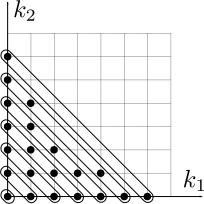
\includegraphics[]{shape_slicing}
    \caption{basic shape (filled bullets) and the slicing (rounded rectangles)}
\end{figure}

The implementation maintains for each slice an array containing all nodes that are part of the slice. The user can decide at compile-time which multi-index type to use:
 \\ \\ A suitable type must \dots
\begin{itemize}
\item \dots provide the same semantics as \code{std::array<int,D>}.
\item \dots specialize \code{std::less} to perform lexical comparison beginning on first index.
\item \dots specialize \code{std::equal\_to} and \code{std::hash}.
\end{itemize}
All nodes inside a slice are ordered according to \code{std::less} of used multi-index type. Be aware that the implemented shape enumerator currently assumes that \code{std::less} performes lexical comparison. Other than that there is nothing inherent that obligates lexical comparison.

\subsection{Enumerator}
A shape enumerator takes a shape object that describes which nodes it contains. The enumerator converts that shape into a shape enumeration.

\subsubsection{Shape Description}
There exists many ways to describe a shape.
The current implementation expects that a shape descriptions exposes two member functions:
\begin{description}
\item [surface description] This member function takes a \emph{base node} \( \underline{n} \) and an \emph{axis} \(j\) and returns the largest element \( k^\star \) that satisfies \( \underline{k}(k^\star) \in \mathfrak{K} \): 
\[ k_i(k^\star) =
\begin{cases}
	n_i,& i \neq j\\
	k^\star, & i = j
	\end{cases}
\]
\item [bounding volume] This member function takes an axis \(j\) and returns an as small as possible \emph{limit} \( L_j \) such that:
\[ \forall \underline{k} \in \mathfrak{K} \,\colon\; k_j \leq L_j \]
\end{description}


Notice that you can describe a shape in another way, but you will need to implement an other shape enumerator.

\begin{figure}[H]
  \centering
  \begin{subfigure}[]{0.4\textwidth}
    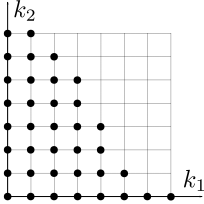
\includegraphics[width=1.0\textwidth]{shape_example}
    \label{fig:shape_example}
  \end{subfigure}
  ~
  \begin{subfigure}[]{0.5\textwidth}
    \begin{tabular}{|| c | c || c | c ||}
      \multicolumn{2}{|| c ||}{\( k_1 \) (first axis) } &
      \multicolumn{2}{c ||}{\( k_2 \) (second axis) } \\
      base node & surface & base node & surface \\
      (?, 0) & 7 & (0, ?) & 7 \\
      (?, 1) & 5 & (1, ?) & 7 \\
      (?, 2) & 4 & (2, ?) & 6 \\
      (?, 3) & 4 & (3, ?) & 5 \\
      (?, 4) & 3 & (4, ?) & 3 \\
      (?, 5) & 3 & (5, ?) & 1 \\
      (?, 6) & 2 & (6, ?) & 0 \\
      (?, 7) & 1 & (7, ?) & 0 \\
      (?, 8) & -1 & (8, ?) & -1 \\
    \end{tabular}
  \end{subfigure}
  \caption{surface description for both axes of a shape example}
\end{figure}

\begin{figure}[htbp]
\centering


\end{figure}

\subsubsection{Enumeration algorithm}
Knowing the \emph{surface} and  \emph{bounding volume} of a shape, the enumerator lexically enumerates all nodes inside the shape. All nodes are subsequently put into the corresponding shape.

\begin{algorithm}[H]
  \For{$x \leftarrow 0$ \KwTo shape.surface($\{0,0,0\}$,$0$)}{
    \For{$y \leftarrow 0$ \KwTo shape.surface($\{x,0,0\}$,$1$)}{
      \For{$z \leftarrow 0$ \KwTo shape.surface($\{x,y,0\}$,$2$)}{
        slice[x+y+z].pushback($\{x,y,z\}$);
      }
    }
  }
  \caption{enumerator passage through a description of a 3D-shape}
\end{algorithm}

\begin{figure}[H]
	\centering
	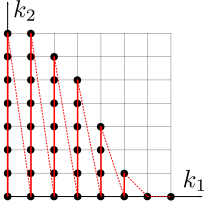
\includegraphics[]{shape_enumerator}
	\caption{enumerator passage through a description of a 2D-shape}
	\label{fig:shape_example}
\end{figure}

\subsection{Abstract Shape Enumeration}

The file \emph{waveblocks/shape\_enumeration\_base.hpp} provides a interface that is meant to be overridden by different implementations. To represent a multi-index, this interface uses the greatest common denominator \emph{std::array\textless int,D\textgreater}. 

\subsection{Default Shape Enumeration}

The file \emph{waveblocks/shape\_enumeration\_default.hpp} provides a default implementation of a shape enumeration.

\begin{verbatim}
template<dim_t D, class MultiIndex, class S>
class DefaultShapeEnumeration;
\end{verbatim}

\begin{description}
\item[D] number of dimensions
\item[MultiIndex] type to internally represent multi-indices
\item[S] shape description
\end{description}

\subsubsection{Internal multi-index representation}
The default shape enumeration stores all nodes in a vector. Since using \emph{std::array\textless int,D\textgreater} would use a lot of memory, the default enumeration exposes a template parameter to define a better type. \\ \\ A suitable type must \dots
\begin{itemize}
\item provide the same semantics as \emph{std::array\textless int,D\textgreater}
\item specialize \emph{std::less} to perform lexical comparison
\item specialize \emph{std::equal\_to}
\item specialize \emph{std::hash}
\end{itemize}

\subsubsection{Shape definition}
A shape definition class provides two member functions:

\begin{itemize}
\item
\begin{verbatim}
int limit(dim_t axis) const;
\end{verbatim}
This member function returns for a given axis \( j \) an as small as possible limit \( L_j \) such that:
\[ \forall \boldsymbol{k} \in \mathfrak{K} \,\colon\; k_j \leq L_j \]

\item
\begin{verbatim}
template<class MultiIndex>
int limit(const MultiIndex &base_node, dim_t axis) const;
\end{verbatim}
This member function for a given axis \( j \) and a given base node \( \boldsymbol{n} \) (whose \( j \)-th entry is zero)
the largest element \( k^\star \) that satisfies: 
\[ \boldsymbol{k} \in \mathfrak{K}, \;
k_i =
   \begin{cases}
      n_i,& i \neq j\\
      k^\star, & i = j
   \end{cases}
\]

\end{itemize}

\subsubsection{Queries}
The default shape enumeration stores all multi-indices in a vector using lexical ordering. The query \emph{ordinal} \(\rightarrow\) \emph{multi-index} is therefore trivial. The query \emph{multi-index} \(\rightarrow\) \emph{ordinal} is done using binary search. Alternatively this implementation can be forced to use \emph{std::unordered\_map} but performance tests revealed that a dictionary is slightly slower than binary seach.

\section{Hagedorn Wavepacket}
A hagedorn wavepacket
\[
\Phi_{\varepsilon}[\Pi] \approx e^{iS\pi} \sum_{\underline{k} \in \mathfrak{K}}^{} c_{\underline{k}} \phi_{\underline{k}} \]
is represented by a tuple
\[ \Phi = \left( \varepsilon, \Pi, \mathfrak{K}, \boldsymbol{c}, S \right) \]
\[ \Pi = \left( \vec{p}, \vec{q}, \mat{P}, \mat{Q} \right) \]

\subsection{Basis Evaluation}

All basis values are evaluated recursively by

\begin{equation}
\label{eq:phi0_Dd}
  \phi_{\mindex{0}}[\Pi]\left(\vec{x}\right)
  \assign
  (\pi\varepsilon^2)^{-\frac{D}{4}} (\det\mat{Q})^{-\frac{1}{2}}
  \exp \left( \frac{i}{2\varepsilon^2}
  \dotp{(\vec{x}-\vec{q})}{\mat{P}\mat{Q}^\mathrm{-1}(\vec{x}-\vec{q})}
  + \frac{i}{\varepsilon^2} \dotp{\vec{p}}{(\vec{x}-\vec{q})}
 \right)
\end{equation}

Having the basis value at a node $\mindex{k}$ we can compute all forward
neighbours by

\begin{equation}
  \begin{pmatrix}
    \phi_{\mindex{k}+\mindex{e}^1} \\
    \vdots \\
    \phi_{\mindex{k}+\mindex{e}^D}
  \end{pmatrix}
  = \left(
  \sqrt{\frac{2}{\varepsilon^2}} \mat{Q}^\mathrm{-1} (\vec{x}-\vec{q}) \phi_{\mindex{k}}
  - \mat{Q}^\mathrm{H} \mat{Q}^\mathrm{-T}
  \begin{pmatrix}
    \sqrt{k_1} \phi_{\mindex{k}-\mindex{e}^1} \\
    \vdots \\
    \sqrt{k_D} \phi_{\mindex{k}-\mindex{e}^D}
  \end{pmatrix}
  \right)
  \oslash
  \begin{pmatrix}
    \sqrt{k_1+1}\\
    \vdots \\
    \sqrt{k_D+1}
  \end{pmatrix}
\end{equation}

where the operator $\oslash$ denotes component-wise division. In a next step
we use this formula for evaluation of all $\phi_{\vec{k}}$ basis functions
of $D$ dimensional semi-classical wavepackets. This last formula is so important
that it should carry a box too but it seems there is no space left.

\begin{figure}[H]
    \centering
    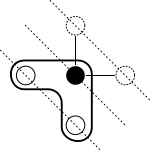
\includegraphics[]{basis_eval_stencil}
    \caption{stencil}
\end{figure}

\begin{algorithm}[H]
 \KwData{this text}
 \KwResult{how to write algorithm with \LaTeX2e }
 \DontPrintSemicolon
 \SetKwInOut{Input}{Input}
 \SetKwInOut{Output}{Output}
 \Input{number of slices $S$}
 \Input{shape enumeration (slices) $\mathfrak{K} = \left(\mathfrak{K}^0, \ldots, \mathfrak{K}^{S-1}\right)$}
 \Output{basis values on each slice $\phi = \left(\phi^0, \ldots, \phi^{S-1}\right)$}
 initialization\;
 $\phi^-, \phi, \phi^+ \gets \emptyset $\;
 
 \emph{Compute ground state}\;
 
 $ \gets \left\{ \phi_{\mindex{0}}[\Pi](\vec{x}) \right\} $\;
 \emph{Loop over all slices}\;
 \ForEach{$\mathfrak{K}^s \in \mathfrak{K}$}{
  \emph{Loop over all nodes of next slice}\;
  \For{$\mindex{k}^{s+1} \in \mathfrak{K}^{s+1}$}{
    \emph{find suitable anchor node (in current slice)}\;
    $a \gets undef $\\
    \For{$d \in {1,\ldots,D}$}{
        \If{$k^{s+1}_{d} > 0$}{
            $a \gets d$\;
        }
    }
    \emph{here is our anchor node $\mindex{k}^{s}$}\;
    $\mindex{k}^{s} \gets \mindex{k}^{s+1} - \mindex{e}^a$\;
    
    \emph{compute contribution of anchor node}\;
    $a \gets \frac{\sqrt{2}}{\varepsilon}\left(\mat{Q}^\mathrm{-1}(\vec{x}-\vec{q})\right)_a\phi^{s}_{\mindex{k}}$
    
    \emph{compute contribution of anchor node's precursors}\;
    $b \gets 0$\;
    \For{$d \in {1,\ldots,D}$}{
        \If{$k^{s}_{d} > 0$}{
            $b \gets b + \sqrt{k^{s}_d} 
                \left(\mat{Q}^{\mathrm{H}}\mat{Q}^{\mathrm{-T}}\right)_{ad}
                \phi^{s-1}_{\mindex{k}^{s}-\mindex{e}^d}$\;
        }
    }
    
    \emph{compute value of basis at $\mindex{k}^{s+1}$}\;
    $\phi^{s+1}_{\mindex{k}^{s+1}} \gets \frac{a-b}{\sqrt{1+k^{s}_a}} $
  }
 }
 \caption{Recursive basis evaluation of hagedorn wavepacket}
\end{algorithm}

\subsection{Applying the Gradient Operator}
For a given wavepacket \( \left(  \right) \)

\[ 
\nabla \left( \varepsilon, \Pi, \mathfrak{K}, \boldsymbol{c} \right) \rightarrow
\left( \varepsilon, \Pi, \mathfrak{K}_{ext}, \boldsymbol{c_\nabla}, \right)
\]

\end{document}
